% CVPR 2026 Paper Template; see https://github.com/cvpr-org/author-kit

\documentclass[10pt,twocolumn,letterpaper]{article}

%%%%%%%%% PAPER TYPE  - PLEASE UPDATE FOR FINAL VERSION
% \usepackage{cvpr}              % To produce the CAMERA-READY version
\usepackage[review]{cvpr}      % To produce the REVIEW version
% \usepackage[pagenumbers]{cvpr} % To force page numbers, e.g. for an arXiv version
\usepackage{float}
% Import additional packages in the preamble file, before hyperref
%% This file contains a number of tweaks that are typically applied to the main document.
%% They are not enabled by default, but can be enabled by uncommenting the relevant lines.

%%
%% Inline annotations; for predefined colors, refer to "dvipsnames" in the xcolor package:
%% https://tinyurl.com/overleaf-colors
%%
\newcommand{\red}[1]{{\color{red}#1}}
\newcommand{\todo}[1]{{\color{red}#1}}
\newcommand{\TODO}[1]{\textbf{\color{red}
[TODO: #1]}}
\newcommand{\methodname}{BELNOME}
\newcommand{\best}[1]{\ensuremath{\boldsymbol{#1}}}
\newcommand{\second}[1]{\ensuremath{\underline{#1}}}
\newcommand{\epre}{\mathrm{EPRE}}
\usepackage{algorithm}
\usepackage{algpseudocode}
%%
%% disable for camera ready / submission by uncommenting these lines  
%%
% \renewcommand{\TODO}[1]{}
% \renewcommand{\todo}[1]{#1}

%%
%% work harder in optimizing text layout. Typically shrinks text by 1/6 of page, enable
%% it at the very end of the writing process, when you are just above the page limit
%%
% \usepackage{microtype}

%%
%% fine-tune paragraph spacing
%%
% \renewcommand{\paragraph}[1]{\vspace{.5em}\noindent\textbf{#1.}}

%%
%% globally adjusts space between figure and caption
%%
% \setlength{\abovecaptionskip}{.5em}


%%
%% Allows "the use of \paper to refer to the project name"
%% with automatic management of space at the end of the word
%%
% \usepackage{xspace}
% \newcommand{\paper}{ProjectName\xspace}

%%
%% Commonly used math definitions
%%
% \DeclareMathOperator*{\argmin}{arg\,min}
% \DeclareMathOperator*{\argmax}{arg\,max}

%%
%% Tigthen underline
%%
% \usepackage{soul}
% \setuldepth{foobar}


% It is strongly recommended to use hyperref, especially for the review version.
% hyperref with option pagebackref eases the reviewers' job.
% Please disable hyperref *only* if you encounter grave issues, 
% e.g. with the file validation for the camera-ready version.
%
% If you comment hyperref and then uncomment it, you should delete *.aux before re-running LaTeX.
% (Or just hit 'q' on the first LaTeX run, let it finish, and you should be clear).
\definecolor{cvprblue}{rgb}{0.21,0.49,0.74}
\usepackage[pagebackref,breaklinks,colorlinks,allcolors=cvprblue]{hyperref}

%%%%%%%%% PAPER ID  - PLEASE UPDATE
\def\paperID{16321} % *** Enter the Paper ID here
\def\confName{CVPR}
\def\confYear{2027}

%%%%%%%%% TITLE - PLEASE UPDATE
\title{MorphCraft3D: A Unified Generative Framework \\for 3D-Conditioned Textured Morphing}

%%%%%%%%% AUTHORS - PLEASE UPDATE
\author{First Author\\
Institution1\\
Institution1 address\\
{\tt\small firstauthor@i1.org}
% For a paper whose authors are all at the same institution,
% omit the following lines up until the closing ``}''.
% Additional authors and addresses can be added with ``\and'',
% just like the second author.
% To save space, use either the email address or home page, not both
\and
Second Author\\
Institution2\\
First line of institution2 address\\
{\tt\small secondauthor@i2.org}
}

\begin{document}
\twocolumn[{%
    \renewcommand\twocolumn[1][]{#1}%
    \maketitle
    \centering
    \includegraphics[width=\textwidth]{figures/figure.pdf}
    \captionof{figure}{Textured 3D morphing with \methodname{}.
The first and second source assets correspond to
$\alpha=1$ and $\alpha=0$, respectively.}
    \label{fig:main}
    \vspace{1em}
}]
\begin{abstract}
Generating plausible transitions between textured 3D objects remains challenging, as geometry and appearance must evolve coherently despite
the absence of ground-truth morphing trajectories. Recent approaches leverage pretrained 3D generative models to synthesize
intermediate states, but rely on predefined interpolation strategies rather than learning how objects should transform across diverse examples.
In this work, we introduce \methodname{}, a framework that turns generated morphing trajectories into supervision for learning a
generalizable 3D morphing function. By training across diverse source objects, our model learns to combine
their geometric and appearance information directly from 3D representations, replacing fixed interpolation rules with adaptive
source conditioning. To mitigate artifacts inherited from generated supervision, we further incorporate a pretrained generative prior that guides the
learning process toward plausible intermediate states. Experiments demonstrate more regular perceptual progression and substantially faster generation than recent training-free approaches, while maintaining competitive visual quality.
\end{abstract}    
\section{Introduction}
\label{sec:introduction}

Morphing transforms one 3D object into another through a sequence of intermediate states, with applications in animation, visual effects, and 3D content creation. Given two textured 3D objects, a successful transition must jointly evolve geometry and appearance, produce plausible intermediate states, and progress smoothly between them. %However, two objects do not define a unique morphing trajectory, as multiple transformations may be equally valid. 
In addition, learning such transitions is further complicated by the lack of ground-truth morphing trajectories, since existing 3D asset collections typically provide individual objects rather than intermediate sequences: for this reason, recent generative approaches use pretrained 3D models to generate intermediate states.
% For this reason, recent generative approaches to textured 3D morphing try to leverage pretrained 3D models to produce intermediate states. 
Interp3D~\cite{liu2026interp3d}, and MorphAny3D~\cite{sun2026morphany3d} build on TRELLIS~\cite{xiang2025trellis}, a pretrained 3D generation method, combining information from two source objects through predefined fusion strategies. Both these methods are training-free and do not learn a reusable morphing function optimized across a collection of example trajectories. However, generated sequences can exhibit artifacts, abrupt changes, or premature convergence toward one object. Moreover, representing source assets through 2D views can discard information about unobserved geometry
before morphing begins. %As a result, the quality of the generated transitions can depend on the viewpoint and quality of the input images.

Despite these limitations, training-free methods can provide a large number of pseudo-trajectories that would otherwise be unavailable for supervised learning. Our key idea is to use these trajectories as pseudo-supervision for learning a morphing function, rather than treating them as final outputs. By training across many source pairs and interpolation coefficients, we obtain a model that learns shared patterns of geometric and appearance transformations instead of relying on predefined fusion procedures. We hypothesize that learning these common patterns can improve generalization to unseen object pairs while reducing some of the irregularities present in the generated trajectories. %teacher-generated trajectories.

To realize this idea, we introduce \methodname{}, a teacher-student framework for textured 3D morphing. First, we use Interp3D as a teacher to generate morphing pseudo-targets of two source objects.
Then, we define a student model that adapts the TRELLIS generation process and learns to combine information from both sources using the teacher supervision. 
Unlike image-driven approaches, our framework conditions directly on the 3D representations of the sources, avoiding the need to reconstruct their geometry from images and the associated ambiguities in unobserved regions. 

However, teacher-generated pseudo-targets may still contain artifacts that could be transferred to the student during training. To mitigate this issue, we introduce a frozen TRELLIS-based generative prior that provides an additional regularization signal, encouraging the student to produce plausible intermediate states rather than merely reproducing the teacher's outputs.

% Our experiments show that \methodname{} produces intermediate morphing states with fewer artifacts and better preservation of source geometry w.r.t. previous training-free approaches. Additionally, the generated trajectories exhibit smoother and more balanced transitions, reducing abrupt changes and premature convergence toward either source object. To evaluate the progression of these transitions, we introduce Source Profile Error (SPE), a source-normalized metric that measures how perceptual changes are distributed along the morphing trajectory. Quantitatively, our method reduces PDV by 39\% compared to the strongest baseline, achieves the lowest SPE under multiple evaluation protocols, and obtains the best FID. Furthermore, once trained, our model requires no pair-specific optimization and generates morphing sequences approximately three times faster than existing approaches.
Evaluating morphing requires assessing both the quality of intermediate states and how the transition progresses between the sources. Measures of individual states or changes between consecutive states do not explicitly capture this source-relative progression. We therefore introduce Source Profile Error (SPE), a source-normalized metric that evaluates progression relative to both input objects. Our experiments against Interp3D and MorphAny3D show more regular perceptual progression and competitive visual quality, together with substantially lower generation time.

The main contributions of this paper are as follows:
\begin{itemize}
    \item We introduce \methodname{}, a teacher-student framework that learns textured 3D morphing from training-free pseudo-trajectories, without requiring exact ground-truth morphing sequences. \methodname{} is conditioned directly on the 3D representations of both source objects using a learned attention fusion mechanism called Gate-Adapted Morphing Cross-Attention (GAMCA).
    \item We introduce a generative regularization strategy based on a frozen TRELLIS prior, complementing teacher supervision to encourage plausible intermediate states.

    \item We propose Source Profile Error (SPE), a source-normalized metric that evaluates progression relative to both source assets, complementing existing quality and smoothness metrics.
\end{itemize}

\section{Related Work}
\label{sec:related}

\subsection{Geometric Shape Morphing}
Geometric approaches construct morphing trajectories from relationships
between the endpoint surfaces. Learned matching and interpolation methods
combine geometric features, optimal transport, and deformation priors to
estimate or refine correspondences without manual
annotations~\cite{eisenberger2020deepshells,eisenberger2021neuromorph,attaiki2023ncp}.
Neural implicit formulations further accommodate noisy inputs and topology
changes without supervision on intermediate shapes~\cite{sang2025fourdeform}.
These advances relax restrictive geometric assumptions, but primarily
address shape evolution rather than the joint synthesis of geometry and
appearance. Bridging geometric and generative approaches,
SRIF~\cite{sun2024srif} lifts multiview image morphs into intermediate point
clouds that guide continuous shape registration. Generated observations
can thus inform geometric trajectories, although jointly synthesizing
shape and texture also requires modeling how appearance evolves.

\subsection{Generative Image Morphing}
Diffusion priors allow morphing to synthesize intermediate content rather
than only deform and blend pixels. Existing approaches interpolate noisy
latents and conditioning signals, often together with endpoint-specific
adaptation or perceptually informed
sampling~\cite{wang2023interpolating,yang2024impus,zhang2024diffmorpher}.
Complementary strategies control feature mixing inside the generator
through attention interpolation, attention fusion, and
correspondence-guided
transport~\cite{he2024aid,cao2025freemorph,shen2024dreammover}.
Together, these works highlight the importance of coordinating global
semantic change with local structure and appearance, rather than relying
on latent interpolation alone. However, a smooth image transition does
not itself define a consistent 3D trajectory: independently lifting
intermediate images into 3D can introduce geometric discontinuities and
inconsistent unobserved surfaces. Transferring these mechanisms
to 3D therefore requires coupling their semantic flexibility with a
representation of the evolving asset.

\subsection{Generative Textured 3D Morphing}
Radiance fields and Gaussian primitives support detailed reconstruction
and rendering~\cite{mildenhall2020nerf,kerbl2023gaussians}, while learned
shape latents and structured Gaussian representations provide shared
spaces for generative
modeling~\cite{zhang2023shape2vecset,zhang2024gaussiancube}.
For textured morphing, volumetric transport and source-adapted diffusion
offer alternatives to explicit surface
deformation~\cite{tsai2022morphflow,Yang_2025_ICCV}.
The former optimizes transitions between multiview reconstructions,
whereas the latter interpolates noise, adapted model parameters, and
conditioning features within a pretrained 3D generator. Both construct
transitions using optimization specific to the input assets.
TRELLIS~\cite{xiang2025trellis} provides a versatile generative space
through structured latents (SLat), separating sparse spatial support from
local geometry and appearance features.

Building on this representation, recent training-free methods coordinate
geometry and texture through optimal transport, progressive alignment,
and attention-based
fusion~\cite{yin2025wukong,liu2026interp3d,sun2026morphany3d}.
WUKONG combines condition interpolation with sequential initialization
and semantic consistency, while Interp3D progressively aligns conditioning
semantics, SLat-guided structure, and appearance. MorphAny3D instead fuses
endpoint information through cross-attention and propagates preceding-frame
features through self-attention, with orientation correction to stabilize
the sequence. It also supports existing assets through 3D inversion.
Although these procedures adapt their outputs to each input pair, they do
not learn a shared morphing function across a collection of transitions.

\methodname{} takes a complementary approach by treating training-free
morphs as supervision rather than as the final inference procedure.
Using Interp3D-generated targets, we learn source fusion across many
object pairs and interpolation coefficients, conditioning both generation
stages directly on the source SLat representations. A separate frozen TRELLIS prior
regularizes the student's own outputs, complementing the example
trajectories supplied by the teacher. This yields a reusable
3D-conditioned morphing model that requires no source-specific parameter
optimization at inference.

\section{Method}
\label{sec:method}

Given two textured 3D assets $S_1$ and $S_2$, our objective is to generate
a continuous morphing sequence controlled by an interpolation coefficient
$\alpha\in[0,1]$, with $\alpha=1$ corresponding to $S_1$ and $\alpha=0$
to $S_2$. We approach this task through a teacher--student framework
that transforms training-free morphing predictions into supervision for
a learnable generative model. By training on morphs produced from many different objects, the student learns a shared morphing function, rather than relying on a fixed interpolation procedure.
An overview of the proposed framework is shown in
Fig.~\ref{fig:architecture}.

\begin{figure*}[t]
 \centering
 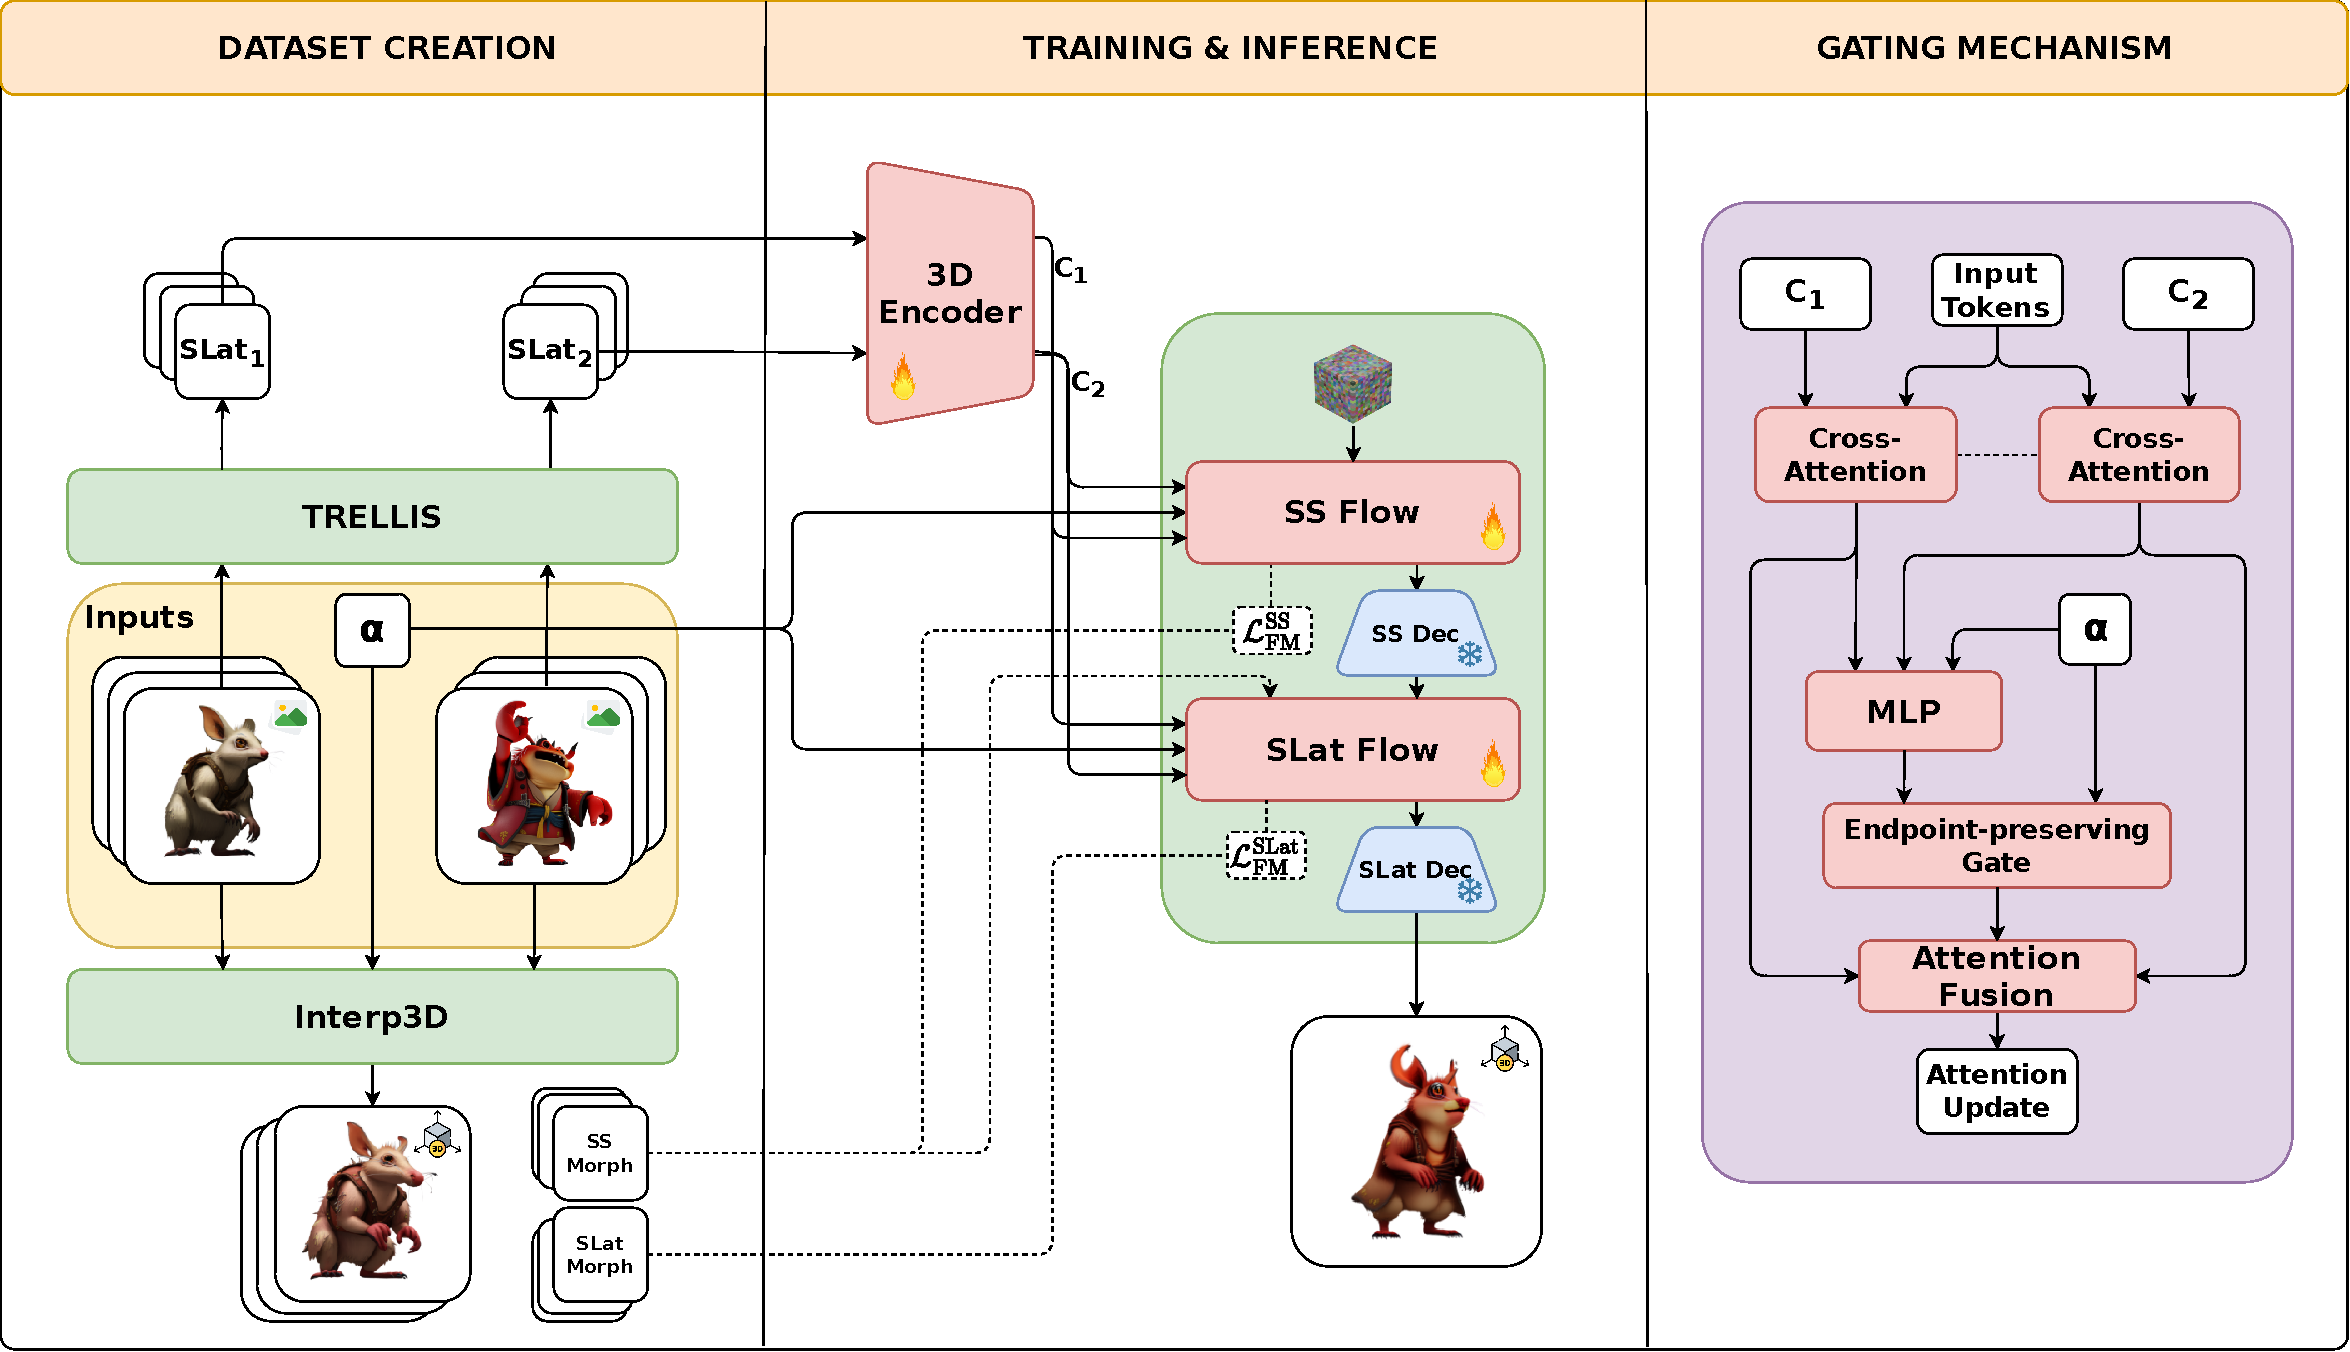
\includegraphics[width=\textwidth]{figures/architecture_overview.pdf}
 \caption{\textbf{Learning textured 3D morphing.} Interp3D produces latent
 targets from source pairs and interpolation coefficients. The student
 encodes each source SLat independently and generates sparse structure and
 structured features. The right panel shows two evaluations of the same
 cross-attention on the source conditions, followed by learned gating.
 Flames mark modules with trainable parameters; snowflakes mark frozen
 decoders. Dashed supervision connections are used during training.}
 \label{fig:architecture}
\end{figure*}

\subsection{Preliminaries}
\label{sec:preliminaries}
%TRELLIS~\cite{xiang2025trellis} is a 3D generation method which represents 3D assets through structured latents (SLat). Instead of encoding an entire object in a single vector, SLat associates local feature vectors with the occupied locations of a sparse 3D grid. The active voxel positions describe the object's spatial support, while the features carried by those positions contain information about its geometry and appearance. This separation makes it possible to model where an object exists in space and what its local structure looks like.
TRELLIS\cite{xiang2025trellis} generates 3D assets conditioned on images or text using structured latents (SLat). In this representation, each active location of a sparse 3D grid carries local features describing geometry and appearance. The representation therefore separates the asset’s spatial support from the information associated with each occupied location.

To generate these latents, TRELLIS uses two successive transformer-based rectified flows~\cite{xiang2025trellis,liu2023rectifiedflow}. First, the sparse-structure (SS) flow predict a latent from which the occupied grid locations are decoded; conditioned on this support, the SLat flow then generates their local features. For image-conditioned generation, DINOv2~\cite{oquab2023dinov2} encodes the input image into visual tokens that condition both flows through cross-attention. The resulting SLat representation can then be decoded into a mesh, 3D Gaussian splats~\cite{kerbl2023gaussians}, or a radiance field~\cite{mildenhall2020nerf}.

Building on this representation, we adapt both the SS and SLat flows within the same morphing framework, adapting them to work with a pair of source 3D assets.

\subsection{Framework}
\subsubsection{Training Dataset Construction}
\label{sec:dataset_construction}
Since ground-truth morphing trajectories are not naturally available, we developed a teacher-student framework, using Interp3D ~\cite{liu2026interp3d} as a teacher to generate the training data for our student model. Because Interp3D is image-conditioned, we start from 12,500 distinct pairs of source images, from which the corresponding 3D assets $S_1,S_2$ are generated. For each pair, we then produce four morphing samples at different interpolation coefficients $\alpha\in[0,1]$, including $\alpha=0$ and $\alpha=1$ to encourage the student to reconstruct the source objects. Finally, we extract the corresponding SS and SLat representations from each generated asset. %, which serve as targets for supervising the two stages of our model. 

Each training example therefore contains the two source SLat representations, an interpolation coefficient, and the teacher-generated SS and SLat latents for that coefficient.%, allowing the student to learn morphing transformations directly in the TRELLIS latent space.

\subsubsection{Architecture}
\label{sec:architecture}
% We define our student model as follows. Using the dataset described in Sec.~\ref{sec:dataset_construction}, we adapt the two generation flows of TRELLIS~\cite{xiang2025trellis} to learn 3D morphing transformations directly from the source representations.

% Given two source assets, the student processes their SLat representations through a 3D encoder $\mathcal E_{3D}$, which extracts spatial information from their coordinates and features. The resulting conditioning tokens are projected into the feature space of the pretrained flow transformers:
To learn morphing from these training examples, our student adapts the two generation flows of TRELLIS~\cite{xiang2025trellis} to use conditions extracted directly from the source 3D assets. Let $z_i$ denote the SLat coordinates and features of asset $S_i$. A shared encoder $\mathcal E_{3D}$ maps $z_i$ to conditioning tokens $c_i$, replacing the image-derived conditions used by the original flows:
\begin{equation}
c_i = \mathcal E_{3D}(S_i),
\qquad i\in{1,2}.
\label{eq}
\end{equation}

\noindent 
so that the student can generate morphs from the source 3D representations.

Each condition contains 4096 tokens arranged on a $16\times16\times16$ grid matching the resolution of the SS representation, with positional embeddings encoding their spatial locations. The 1024-dimensional features match the dimensionality of the DINOv2 embeddings used to condition the pretrained TRELLIS cross-attention layers.

Starting from the pretrained TRELLIS weights, we optimize LoRA adapters~\cite{hu2022lora} together with the 3D encoder and the gate network used in the Gate-Adapted Morphing Cross-Attention (GAMCA). Within each transformer block, a gate network $\mathcal G$ learns to combine the responses of a shared cross-attention module to the two source conditions, as described in Sec.~\ref{sec:attention_gating}.


%Obtaining intermediate ground-truth assets for arbitrary  morphing sequences is inherently difficult: we address this lack of supervision by using Interp3D~\cite{liu2026interp3d} as a training-free teacher. Given a pair of assets and an interpolation coefficient, the teacher produces a morph that serves as pseudo-target for the corresponding student generation, allowing us to train on a collection of transitions. By learning shared morphing patterns across diverse objects, the student can generalize beyond individual teacher predictions, reducing teacher-specific artifacts and producing more coherent transitions. The student architecture is structured as follows: (a) a TRELLIS backbone finetuned using LoRA~\cite{hu2022lora}, (b) a 3D encoder $\mathcal{E}_{3D}$ providing the conditions for both TRELLIS flows and (c) an attention gate $\mathcal{G}$ which learns to combine the assets. During training, the teacher supplies intermediate SS and SLat pseudo-targets for source pairs and interpolation coefficients. These pseudo pairs are then encoded  independently using the encoder $\mathcal{E}_{3D}$ that adapts them to be compatible with TRELLIS conditioning mechanism and produces the encoded representations $c_1$ and $c_2$. Finally, $\mathcal{G}$ combines these representations using the coefficient $\alpha$. As teacher, we selected Interp3D~\cite{liu2026interp3d} as it currently represents the best trade off between generation quality and computational efficiency.

% \subsubsection{Learning from latent pseudo-targets}
% \label{sec:teacher_supervision}
% We train the SS and SLat flows with conditional flow matching~\cite{lipman2022flowmatching}, using the teacher-generated latents as supervision. For either stage, let $z_0$ denote the target latent for a source pair and interpolation coefficient $\alpha$. We sample Gaussian noise $\epsilon\sim\mathcal N(0,I)$ and a noise time $\tau\in[0,1]$, and construct
% \begin{align}
%  z_\tau &=(1-\tau)z_0+\sigma_\tau\epsilon,
%  \label{eq:fm_path}\\
%  \sigma_\tau &=\sigma_{\min}+(1-\sigma_{\min})\tau,\nonumber\\
%  u_\tau &=(1-\sigma_{\min})\epsilon-z_0,
%  \nonumber
% \end{align}
% where $\sigma_{\min}$ is a small positive constant controlling the
% residual noise at the data endpoint. Here, $\tau$ specifies the noise
% level, whereas $\alpha$ specifies the position along the morphing
% sequence. The student learns to predict the target velocity $u_\tau$
% from the perturbed latent and the two source conditions:
% \begin{equation}
%  \mathcal L_{\mathrm{FM}}=
%  \mathbb E\!\left[
%  \left\|v_\theta(z_\tau,\tau;c_1,c_2,\alpha)-u_\tau\right\|_2^2
%  \right].
%  \label{eq:flow_matching}
% \end{equation}
% The expectation is over training examples, noise, and noise times.
% To encourage consistency with respect to source ordering, we also
% swap the two sources and replace $\alpha$ with $1-\alpha$, retaining
% the same teacher-generated target.

% Interp3D~\cite{liu2026interp3d} supplies intermediate SS and SLat
% pseudo-targets for source pairs and interpolation coefficients.
% The student retains both TRELLIS flows but conditions them directly on
% the source assets. An asset encoder processes the features and coordinates
% of each source SLat independently, producing $c_1,c_2$.
% LoRA~\cite{hu2022lora} adapts the pretrained flow parameters, while the
% source encoder and attention gate learn to combine the assets.

% In order to finetune our student, conditional flow matching~\cite{lipman2022flowmatching} is used to train each flow against its teacher latents. Let $z_0$ be a target, $\epsilon$ Gaussian noise, $\tau$ the noise timestep and $\sigma_{\min}$ is a small positive hyperparameter controlling the residual noise at the data endpoint. The training path and target velocity are
% \begin{align}
% z_\tau &=(1-\tau)z_0+
%       [\sigma_{\min}+(1-\sigma_{\min})\tau]\epsilon,\\
% u_\tau &=(1-\sigma_{\min})\epsilon-z_0,
% \end{align}
% with objective
% \begin{equation}
% \mathcal L_{\mathrm{FM}}=
% \mathbb E\|v_\theta(z_\tau,\tau;c_1,c_2,\alpha)-u_\tau\|_2^2.
% \end{equation}
% Sampling integrates the learned field from noise toward the latent data. To enforce consistency across source orderings, each training example is augmented by swapping the two source assets and replacing $\alpha$ with $1-\alpha$, while retaining the same teacher-generated target.

\subsubsection{Gate-Adapted Morphing Cross-Attention}
\label{sec:attention_gating}
GAMCA combines the responses of the cross-attention module to the two source conditions through a learnable gate. While the interpolation coefficient $\alpha$ controls the overall balance between the sources, the gate adjusts their relative contributions across latent tokens and feature channels, allowing different parts of the morph to combine source features differently. The same mechanism is applied in both the SS and SLat generation stages, where each transformer block processes latent tokens $x\in\mathbb R^{N\times d}$ with $d=1024$.

The SS flow operates on a fixed set of $N=4096$ tokens, whereas the SLat flow processes a variable number of active tokens, determined by the asset's spatial support at the transformer resolution.
In either case, the current latent are provided to the cross-attention operator, denoted by $\operatorname{CA}$, which is evaluated separately on the two source conditions:
% First of all, two evaluations of the cross-attention module produce source-specific responses:
\begin{equation}
 h_1=CA(x,c_1),\qquad h_2=CA(x,c_2),
\end{equation}
The resulting responses $h1, h2$ are then combined using weights that adapt to their features and to the interpolation coefficient $\alpha$:
\begin{equation}
 \begin{aligned}
  \delta &=\mathcal G(h_1,h_2,\alpha),\\
  g &=(1-\alpha)+\alpha(1-\alpha)\tanh(\delta),\\
  x &\leftarrow x+(1-g)\odot h_1+g\odot h_2,
 \end{aligned}
 \label{eq:attention_gate}
\end{equation}
where $\mathcal G$ is an MLP that predicts the residual adjustment $\delta$, while $g$ contains the resulting mixing weights. Both $\delta$ and $g$ have the same dimensions as $x$, and $\odot$ denotes elementwise multiplication.

We initialize $\mathcal G$ to output zero, so the fusion initially reduces to $\alpha h_1+(1-\alpha)h_2$. As training progresses, the network learns to adjust this mixture according to the source responses and the current generation state. Because the adjustment is multiplied by $\alpha(1-\alpha)$, it vanishes at $\alpha=0$ and $\alpha=1$, leaving only $h_2$ or $h_1$, respectively. At these coefficient values, generation therefore uses only the corresponding source condition, while reconstruction is learned from the teacher targets.
% In order to define a fusion mechanism that can both perform the morphing while maintaining exact endpoints reconstruction we defined an attention gating mechanism which is shared in both generation flows.

% Specifically, within each attention block, the current tokens $x$ attend independently to the two source conditions through cross-attention:
% \begin{equation}
%  h_1=A_\theta(x,c_1),\qquad h_2=A_\theta(x,c_2).
% \end{equation}

% The two attention responses are then fused through a token- and channel-wise gate:
% \[
% \begin{aligned}
% \delta &= \operatorname{MLP}(h_1,h_2,\alpha),\\
% g &= (1-\alpha)+\alpha(1-\alpha)\tanh(\delta),\\
% x &\leftarrow x+(1-g)\odot h_1+g\odot h_2.
% \end{aligned}
% \]

% The MLP is initialized to produce zero outputs, so the fusion initially reduces to \(\alpha h_1+(1-\alpha)h_2\). During training, the learned residual adaptively adjusts the contributions of each source, while the factor \(\alpha(1-\alpha)\) ensures that the correction vanishes at both endpoints, preserving single-source conditioning.
\subsubsection{Training and generative-prior regularization}
\label{sec:teacher_supervision}
\label{sec:generative_prior}

We train the SS and SLat flows using the standard conditional flow-matching objective~\cite{lipman2022flowmatching}, denoted by $\mathcal L_{\mathrm{FM}}$, with the teacher-generated latents as targets. Each target is associated with a source pair and an interpolation coefficient $\alpha$. During training, we also swap the sources and replace $\alpha$ with $1-\alpha$, keeping the target unchanged to encourage consistency with respect to source ordering.

To complement this supervision, we use a generative prior that acts on samples produced by the student. For each stage, the prior is provided by a separate copy of the original image-conditioned TRELLIS flow, kept frozen throughout training. It uses the source images $I_1$ and $I_2$ from which the training assets $S_1$ and $S_2$ were obtained.

We first generate a latent $\hat z$ by running the student's complete sampling procedure from Gaussian noise, conditioned on $c_1$, $c_2$, and $\alpha$. Once generation is complete, we perturb $\hat z$ with fresh Gaussian noise at a sampled noise level, following the TRELLIS noise schedule. The frozen flow then evaluates this same perturbed sample twice, using the DINOv2 embedding~\cite{oquab2023dinov2} of $I_1$ in one evaluation and that of $I_2$ in the other. Each predicted velocity is converted into an estimate of the clean latent under the corresponding source-image condition. To obtain the regression targets $\tilde z_1$ and $\tilde z_2$, we adjust $\hat z$ toward each estimate. We limit the size of each adjustment so that the targets remain close to the student's generated sample.

The prior loss encourages the student output to approach these targets, with $\alpha$ determining the contribution of each source:
\begin{equation}
 \mathcal L_{\mathrm{prior}}=
 \mathbb E\!\left[
 \frac{\alpha}{2}\operatorname{MSE}(\hat z,\tilde z_1)
 +\frac{1-\alpha}{2}\operatorname{MSE}(\hat z,\tilde z_2)
 \right].
 \label{eq:prior}
\end{equation}
At $\alpha=1$, only the term associated with $S_1$ remains, while at $\alpha=0$ only the term associated with $S_2$ remains. The targets are treated as fixed during backpropagation: gradients pass through $\hat z$ to update the student's trainable modules, without differentiating through the target computation. The original TRELLIS flow remains frozen.

The overall objective combines teacher supervision and generative regularization:
\begin{equation}
 \mathcal L=\mathcal L_{\mathrm{FM}}
 +\lambda_{\mathrm{prior}}\mathcal L_{\mathrm{prior}},
\end{equation}
where $\lambda_{\mathrm{prior}}$ controls the contribution of the prior. The frozen flows and source images are needed only during training.

Algorithm~\ref{alg:generative_prior} summarizes the training
procedure, applied to either the SS or SLat flow.

\begin{algorithm}[t]
\caption{Training with a frozen generative prior}
\label{alg:generative_prior}
\small
\begin{algorithmic}[1]
\Require Source conditions $c_1,c_2$, images $I_1,I_2$,
coefficient $\alpha$
\Require Frozen TRELLIS flow $T$, teacher-supervised loss
$\mathcal L_{\mathrm{FM}}$, prior weight $\lambda_{\mathrm{prior}}$

\Statex \textit{Generate a student sample.}
\State Generate $\hat z$ by completing student sampling from
Gaussian noise, conditioned on $(c_1,c_2,\alpha)$

\Statex \textit{Build fixed targets without gradient tracking.}
\State Sample a noise level $\tau$
\State Perturb $\hat z$ with fresh Gaussian noise at level $\tau$,
using the TRELLIS noise schedule, to obtain $\hat z_\tau$
\For{$i\in\{1,2\}$}
    \State $v_i \gets
    T(\hat z_\tau,\tau;\operatorname{DINOv2}(I_i))$
    \State Convert $v_i$ into a clean-latent estimate $\bar z_i$
    \State $\Delta_i \gets \bar z_i-\hat z$
    \If{the magnitude of $\Delta_i$ exceeds its limit}
        \State Reduce the magnitude of $\Delta_i$,
        keeping its direction
    \EndIf
    \State $\tilde z_i \gets \hat z+\Delta_i$
\EndFor

\Statex \textit{Compute the loss and update the student.}
\State $\mathcal L_i \gets
\tfrac12\operatorname{MSE}(\hat z,\tilde z_i)$,
for $i\in\{1,2\}$
\State $\mathcal L_{\mathrm{prior}} \gets
\alpha\mathcal L_1+(1-\alpha)\mathcal L_2$
\State $\mathcal L \gets
\mathcal L_{\mathrm{FM}}
+\lambda_{\mathrm{prior}}\mathcal L_{\mathrm{prior}}$
\State Update the student's trainable parameters using
$\mathcal L$, treating $\tilde z_1,\tilde z_2$ as fixed targets
\end{algorithmic}
\end{algorithm}

% \subsubsection{Generative-prior regularization via frozen flow predictions}
% \label{sec:generative_prior}

% Teacher supervision provides examples of transitions, but it does not
% directly assess the samples generated by the student. We therefore add a
% generative prior that acts on the student's own outputs during training.

% Starting from Gaussian noise $\eta$, we integrate the student flow under
% the two source conditions and the interpolation coefficient, obtaining
% $\hat z=G_\theta(\eta;c_1,c_2,\alpha)$. 

% Then, we perturb the generated latent with fresh Gaussian noise $\epsilon$ at
% a sampled noise time $\tau$:
% \begin{equation}
%  z_\tau=(1-\tau)\hat z+\sigma_\tau\epsilon,
%  \qquad
%  \sigma_\tau=\sigma_{\min}+(1-\sigma_{\min})\tau.
% \end{equation}
% The frozen, image-conditioned TRELLIS flow evaluates this same perturbed
% sample twice, using the DINOv2 embedding~\cite{oquab2023dinov2} of $I_1$
% in one evaluation and that of $I_2$ in the other. Each predicted velocity
% provides an estimate of the clean latent under its source-image
% condition. A bounded local correction derived from that estimate defines
% a nearby regression target $\tilde z_i$ for the student sample.
% The two targets therefore express how the same generated asset should
% change under the two source conditions.

% The source-conditioned prior loss combines these regression errors:
% \begin{equation}
%  \mathcal L_{\mathrm{prior}}=
%  \mathbb E\!\left[
%  \frac{\alpha}{2}\operatorname{MSE}(\hat z,\tilde z_1)
%  +\frac{1-\alpha}{2}\operatorname{MSE}(\hat z,\tilde z_2)
%  \right].
%  \label{eq:prior}
% \end{equation}
% \noindent, with the interpolation coefficient $\alpha$ setting
% the relative influence of the two source-conditioned corrections. At
% $\alpha=1$ only the first term remains, and at $\alpha=0$ only the
% second remains. TRELLIS receives one source image at a time; the
% interpolation coefficient combines the two losses rather than the image
% embeddings.
% The student's trainable modules are updated, while TRELLIS
% remains frozen.

% The complete training objective is
% \begin{equation}
%  \mathcal L=\mathcal L_{\mathrm{FM}}
%  +\lambda_{\mathrm{prior}}\mathcal L_{\mathrm{prior}},
% \end{equation}
% where $\lambda_{\mathrm{prior}}$ controls the influence of the
% generative feedback relative to teacher supervision.



\section{Metrics}
\label{sec:endpoint_metrics}
\begin{figure}[t]
 \centering
 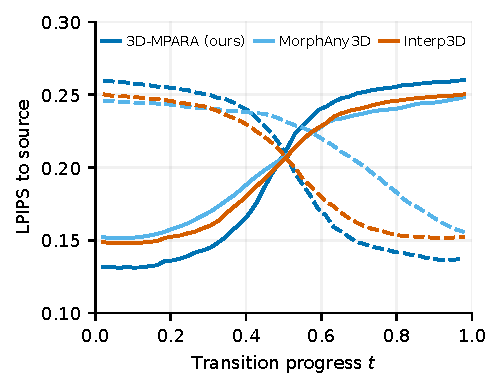
\includegraphics[width=\columnwidth]{figures/endpoint_distances_50.pdf}
 \caption{\textbf{Distances to both sources.} Color identifies the method;
 solid and dashed curves measure LPIPS to source 1 and source 2.
 Each curve averages 64 views over 50 pairs and displays the 48 generated
 intermediates. The canonical endpoint samples are omitted, with no
 connecting segments to $t=0$ or $t=1$.}
 \label{fig:distances50}
\end{figure}

We adopt the Interp Protocol from our teacher,
Interp3D~\cite{liu2026interp3d}, reporting FID~\cite{heusel2017fid} and
Interp3D's adaptation of perceptual path length (PPL)~\cite{karras2019stylegan}.
We also report perceptual distance variance (PDV) from
DiffMorpher~\cite{zhang2024diffmorpher}. FID compares concatenated renders
of two selected intermediates against those of both sources within each pair.
We also report mean LPIPS~\cite{zhang2018lpips} between consecutive
states along the complete path, including both canonical sources.

\begin{table*}[t]
\centering
\small
\setlength{\tabcolsep}{3pt}
\caption{Comparison on 50 held-out pairs. Values are means; \textbf{bold} and \underline{underline} mark the best and second mean in each column. FID, PPL, LPIPS, and PDV use the Interp Protocol; EPRE and TIME report both protocols. LPIPS, PPL, PDV, and EPRE include canonical endpoints. FID uses the concatenated-state definition. PDV is reported in units of $10^{-3}$. TIME is generation time per sequence in seconds. All metrics are minimized.}
\label{tab:standard}
\begin{tabular}{lrrrrrrrr}
\toprule
Method & FID $\downarrow$ & PPL $\downarrow$ & LPIPS $\downarrow$ & PDV ($10^{-3}$) $\downarrow$ & \multicolumn{2}{c}{EPRE $\downarrow$} & \multicolumn{2}{c}{TIME (s) $\downarrow$} \\
\cmidrule(lr){6-7}\cmidrule(lr){8-9}
& & & & & Interp Protocol & Dense Protocol & Interp Protocol & Dense Protocol \\
\midrule
MorphAny3D & \second{95.95} & \best{2.87} & \best{0.118} & $4.88$ & $0.33$ & $0.39$ & \second{182} & $1914$ \\
Interp3D & $96.02$ & \second{3.31} & \second{0.137} & \second{1.40} & \second{0.27} & \second{0.35} & $188$ & \second{897} \\
\methodname{} (ours) & \best{95.03} & $3.58$ & $0.148$ & \best{0.85} & \best{0.26} & \best{0.32} & \best{61} & \best{553} \\
\bottomrule
\end{tabular}
\end{table*}


\subsection{Endpoint Profile Error}
\label{sec:epre}

Image quality and local path regularity do not specify where an
intermediate lies close to its sources as the coefficient changes.
A sequence can change smoothly while staying close to one source or
departing from both. Our results illustrate this distinction: similar FID
and different PPL scores accompany distinct source-distance
profiles (Table~\ref{tab:standard}). The
qualitative sequences in Figure~\ref{fig:qualitative} and distance curves
in Figure~\ref{fig:distances50} motivate examining how each transition
leaves one source and approaches the other.

We introduce endpoint profile error (EPRE) to measure this progression.
Let $M(t)$ be the generated asset at progress $t\in[0,1]$, from $S_1$ to
$S_2$, and let $d(A,B)$ denote LPIPS averaged over matched camera views.
We normalize the distance to each source by their mutual distance:
\begin{equation}
 r_i(t)=\frac{d(M(t),S_i)}{d(S_1,S_2)},\qquad i\in\{1,2\}.
\end{equation}
A linear reference moves from distances $(0,1)$ to $(1,0)$, so its values
at progress $t$ are $(t,1-t)$. Writing $r_i=r_i(t)$, EPRE summarizes the
deviation from this reference across the transition:
\begin{equation}
 \epre=\sqrt{\tfrac12\!\int_0^1
       \big[(r_1-t)^2+(r_2-(1-t))^2\big]\,dt}.
 \label{eq:epre}
\end{equation}
Lower values mean closer agreement with the prescribed progression.
Normalization makes the score relative to the perceptual separation of
each source pair. We integrate over the sampled states using the
trapezoidal rule, including the canonical endpoints, and then average
pair scores.

EPRE complements the existing metrics: it describes source-relative
progression rather than image realism, geometric validity, or a unique
correct morph. The Dense Protocol samples the same reference more
densely, exposing behavior near the endpoints that the five central
intermediates of the Interp Protocol can miss.


\section{Experiments}
\label{sec:experiments}

\subsection{Experimental Setup}

We evaluate \methodname{} against Interp3D~\cite{liu2026interp3d} and MorphAny3D~\cite{sun2026morphany3d} on 50 held-out source pairs. To ensure a controlled comparison, all methods use identical endpoint SLat representations generated by TRELLIS~\cite{xiang2025trellis} with the same code, configuration, and random seeds. All generated assets are evaluated using a common Gaussian renderer with matched cameras.

We adopt the Interp Protocol of Interp3D, consisting of five intermediates sampled at deterministic $\operatorname{Beta}(5,5)$ quantiles and two canonical endpoints. We additionally use the Dense Protocol \citep{sun2026morphany3d} with 48 uniformly spaced intermediates at $t=k/49$, yielding 50 states including the endpoints. LPIPS-based distances are evaluated over 64 matched views, while FID uses 1,000 views per state and two intermediate states selected identically for all methods. FID, PPL, and PDV follow the Interp Protocol, whereas EPRE is evaluated under both protocols. This evaluation applies the Interp3D protocol to our held-out pairs rather than reproducing the Interp3DData leaderboard.

\subsection{Quantitative Results}

\begin{table*}[t]
\centering
\small
\setlength{\tabcolsep}{3pt}
\caption{Comparison on 50 held-out pairs. Values are means; \textbf{bold} and \underline{underline} mark the best and second mean in each column. FID, PPL, LPIPS, and PDV use the Interp Protocol; EPRE and TIME report both protocols. LPIPS, PPL, PDV, and EPRE include canonical endpoints. FID uses the concatenated-state definition. PDV is reported in units of $10^{-3}$. TIME is generation time per sequence in seconds. All metrics are minimized.}
\label{tab:standard}
\begin{tabular}{lrrrrrrrr}
\toprule
Method & FID $\downarrow$ & PPL $\downarrow$ & LPIPS $\downarrow$ & PDV ($10^{-3}$) $\downarrow$ & \multicolumn{2}{c}{EPRE $\downarrow$} & \multicolumn{2}{c}{TIME (s) $\downarrow$} \\
\cmidrule(lr){6-7}\cmidrule(lr){8-9}
& & & & & Interp Protocol & Dense Protocol & Interp Protocol & Dense Protocol \\
\midrule
MorphAny3D & \second{95.95} & \best{2.87} & \best{0.118} & $4.88$ & $0.33$ & $0.39$ & \second{182} & $1914$ \\
Interp3D & $96.02$ & \second{3.31} & \second{0.137} & \second{1.40} & \second{0.27} & \second{0.35} & $188$ & \second{897} \\
\methodname{} (ours) & \best{95.03} & $3.58$ & $0.148$ & \best{0.85} & \best{0.26} & \best{0.32} & \best{61} & \best{553} \\
\bottomrule
\end{tabular}
\end{table*}


Table~\ref{tab:standard} compares the three methods in terms of intermediate quality, perceptual path properties, endpoint progression, and computational efficiency. All methods achieve comparable FID scores, with \methodname{} obtaining the lowest value. Although our method has a higher PPL, indicating a longer perceptual path, it achieves the lowest PDV, reducing it by 39\% compared to Interp3D. This suggests that our method distributes perceptual changes more uniformly along the transition, despite traversing a longer path. In contrast, shorter perceptual paths do not necessarily imply more regular transitions.

Our method also achieves the lowest EPRE under both evaluation protocols, indicating closer agreement with the reference endpoint progression. The improvement is particularly evident under the Dense Protocol, where EPRE decreases from 0.35 for Interp3D to 0.32 for our method. Figure~\ref{fig:epre_profile} provides a more detailed analysis, showing that our method generally produces lower profile errors, particularly near the endpoints, while remaining comparable to Interp3D around the midpoint.

\begin{figure}[t]
    \centering
    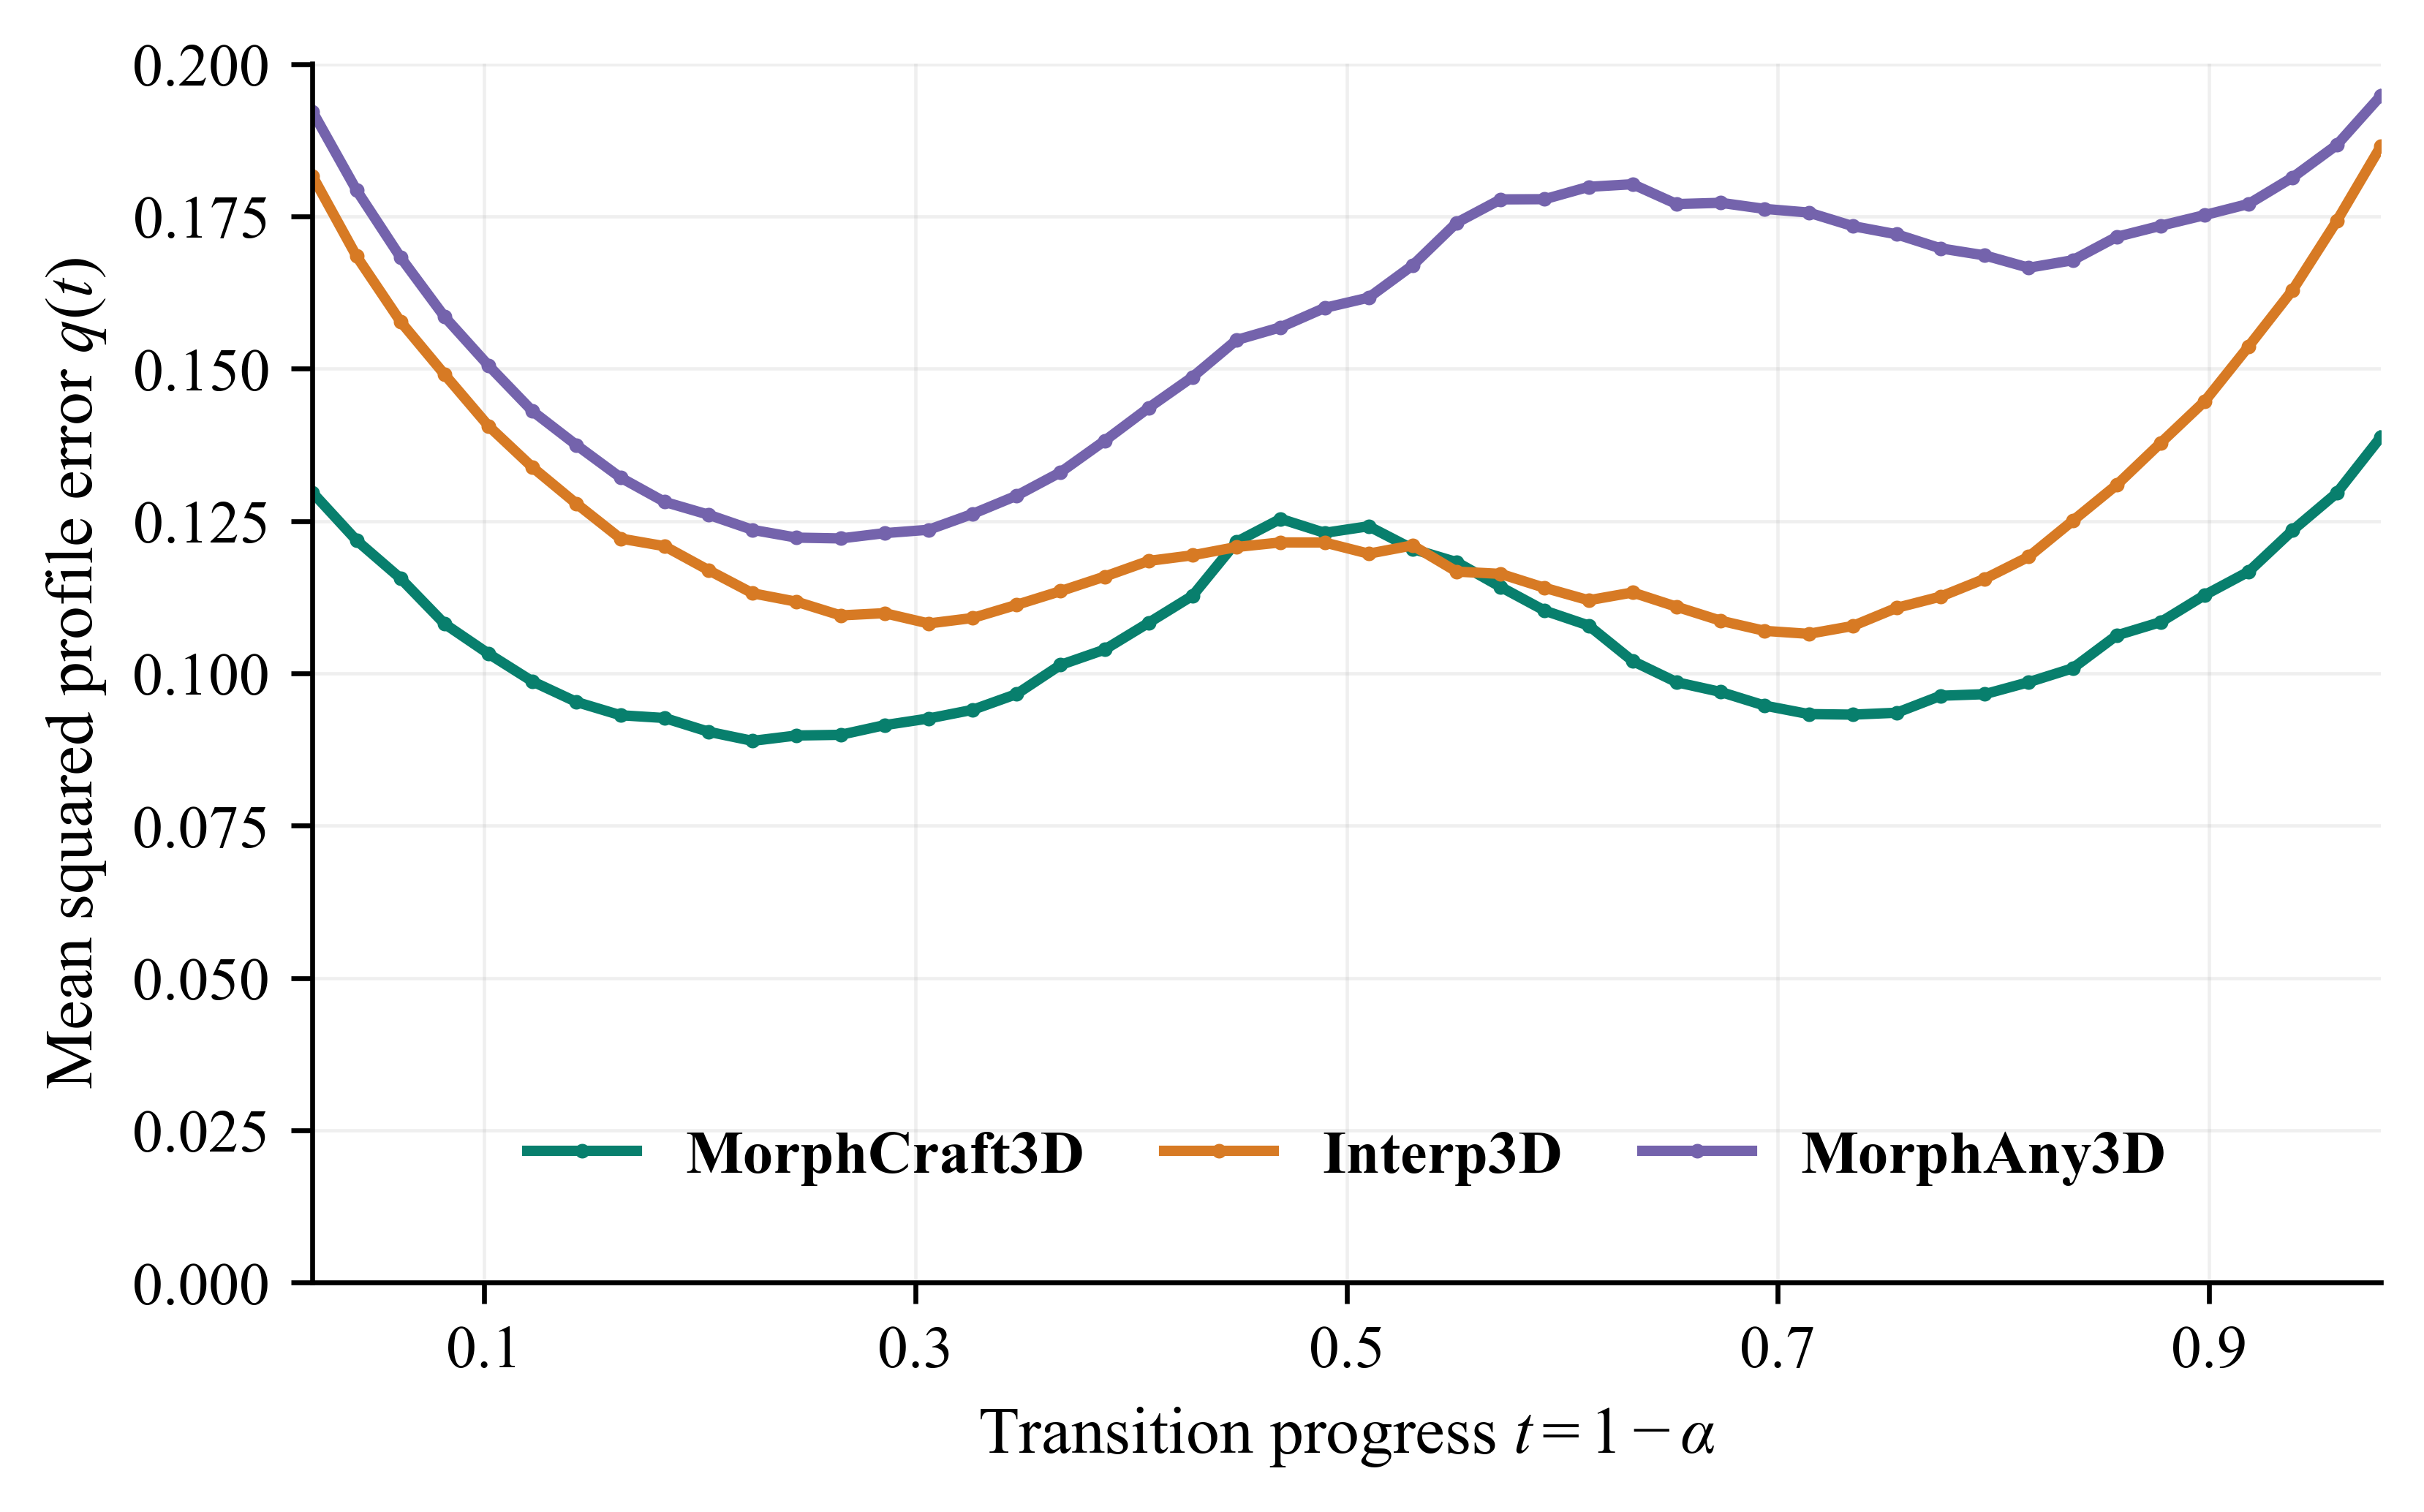
\includegraphics[width=\columnwidth]{figures/epre.png}
    \caption{\textbf{Instantaneous squared endpoint profile error.}
    Mean $q(t)$ over 50 pairs.  Lower values indicate closer agreement with the linear reference.}
    \label{fig:epre_profile}
\end{figure}

Finally, \methodname{} achieves the lowest measured generation time under both protocols. Under the Interp Protocol, it requires 61 seconds per sequence, compared to 188 seconds for Interp3D and 182 seconds for MorphAny3D. The advantage remains under the Dense Protocol, where our method requires 553 seconds compared to 897 and 1914 seconds, respectively.

\subsection{Qualitative Results}

\subsection{Ablation Studies}
\label{sec:ablations}


% \section{Experiments}
% \label{sec:experiments}

% The comparison uses the same 50  source pairs, and a common Gaussian renderer with matched cameras. The
% Interp Protocol follows Interp3D and contains seven states: two canonical sources and five
% intermediates at deterministic $\operatorname{Beta}(5,5)$ quantiles.
% LPIPS uses 64 views; FID uses 1,000 views per state and two intermediate
% states selected identically for all methods. The Dense Protocol generates
% 48 uniform intermediates at $t=k/49$, for 50 states in total, to resolve
% behavior near the endpoints. Only EPRE and generation time are available
% for the Dense Protocol. This evaluates the teacher protocol on our
% pairs, rather than reproducing the Interp3DData leaderboard.

% \subsection{Comparison}
% Table~\ref{tab:standard} compares \methodname{},
% MorphAny3D~\cite{sun2026morphany3d}, and Interp3D~\cite{liu2026interp3d}.
% The methods obtain similar FID means. \methodname{} has lower PDV but a
% longer perceptual path, indicating more uniform step magnitudes while
% traversing a greater total distance. Under the Dense Protocol it obtains
% the lowest mean EPRE. Generation time includes preparation and raw-asset
% serialization, excluding one-time model loading and metric rendering.

% Figure~\ref{fig:distances50} shows how each method moves away from one
% source and approaches the other. Reading both distances together
% distinguishes a transition that stays close to one source from one that
% departs from both. Figure~\ref{fig:qualitative} complements these averages
% with matched views of geometry and appearance.

% \begin{figure*}[t]
%  \centering
%  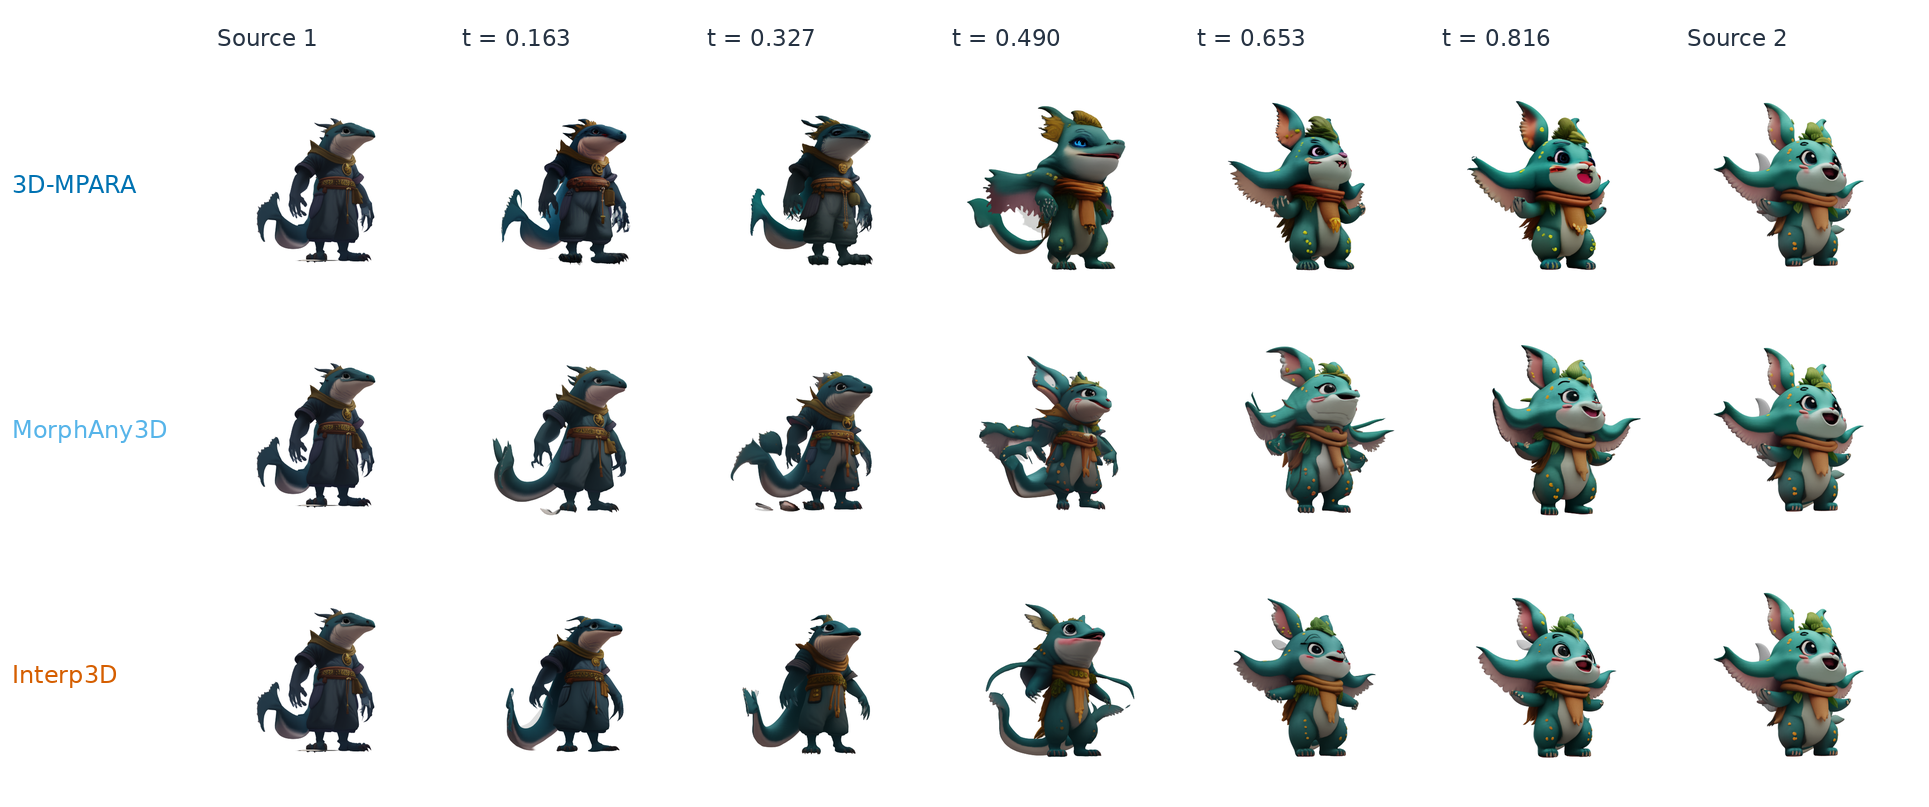
\includegraphics[width=.94\textwidth]{figures/qualitative_pair_0000.png}\\[3pt]
%  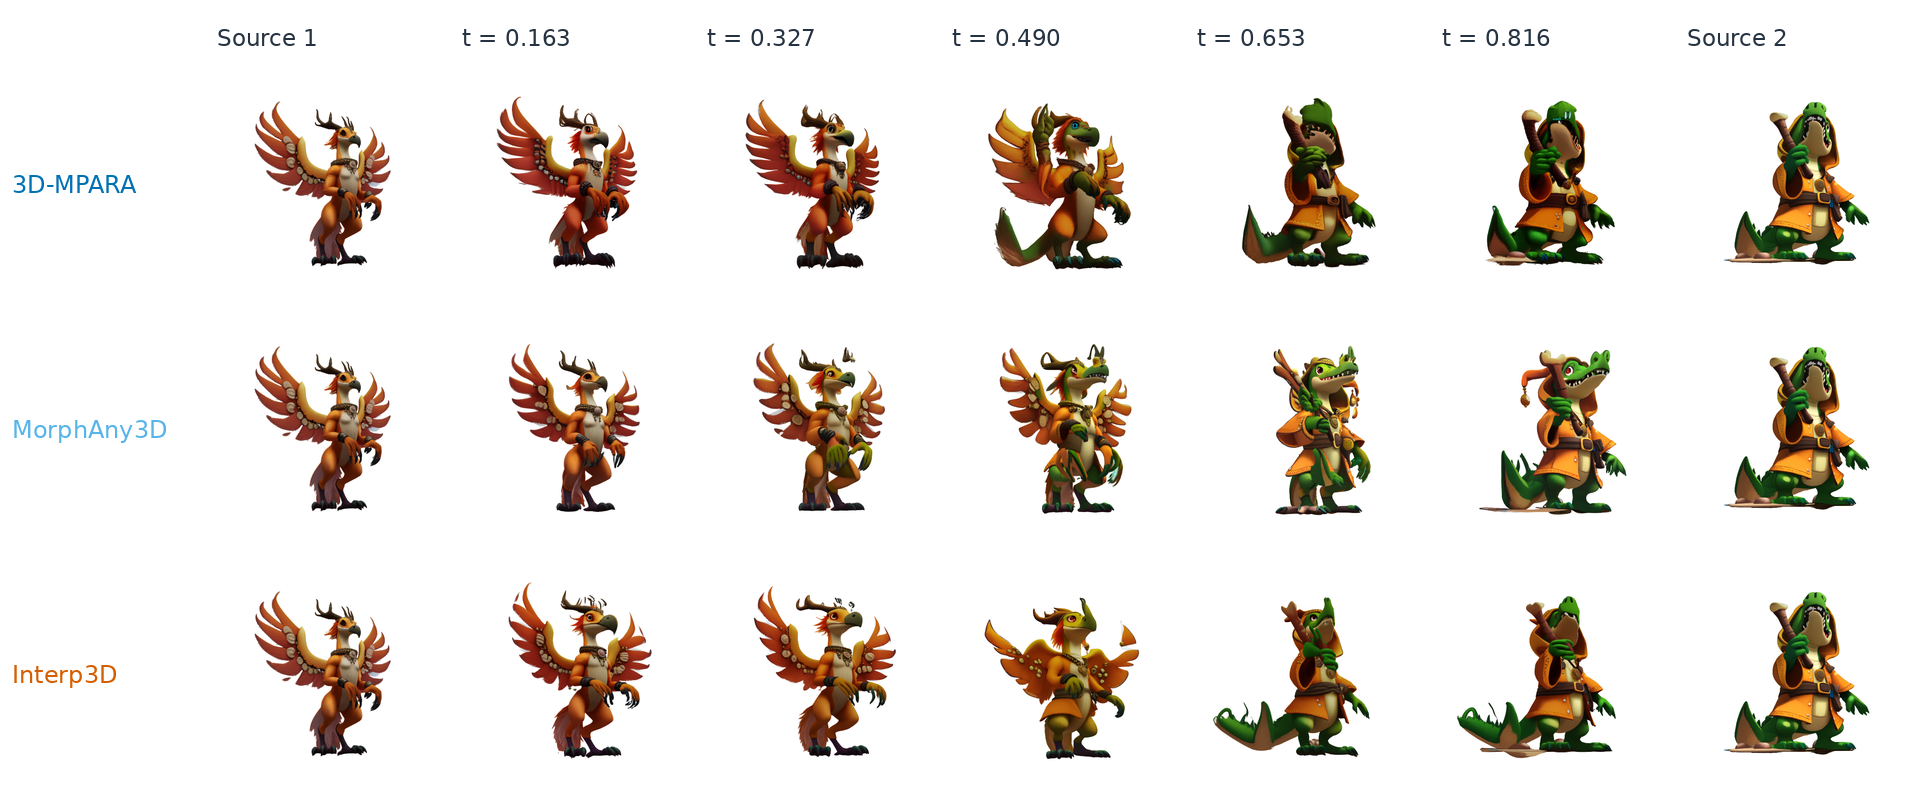
\includegraphics[width=.94\textwidth]{figures/qualitative_pair_0001.png}
%  \caption{\textbf{Textured morphing comparisons.} Each pair has one row per
%  method and a fixed camera (view 025). Columns show seven samples from the
%  dense sequences at $t=0,8/49,16/49,24/49,32/49,40/49,1$.
%  Sources are common canonical assets. These are the first two pairs in
%  the test plan, selected without metric ranking.}
%  \label{fig:qualitative}
% \end{figure*}

% \begin{figure}[h]
%  \centering
%  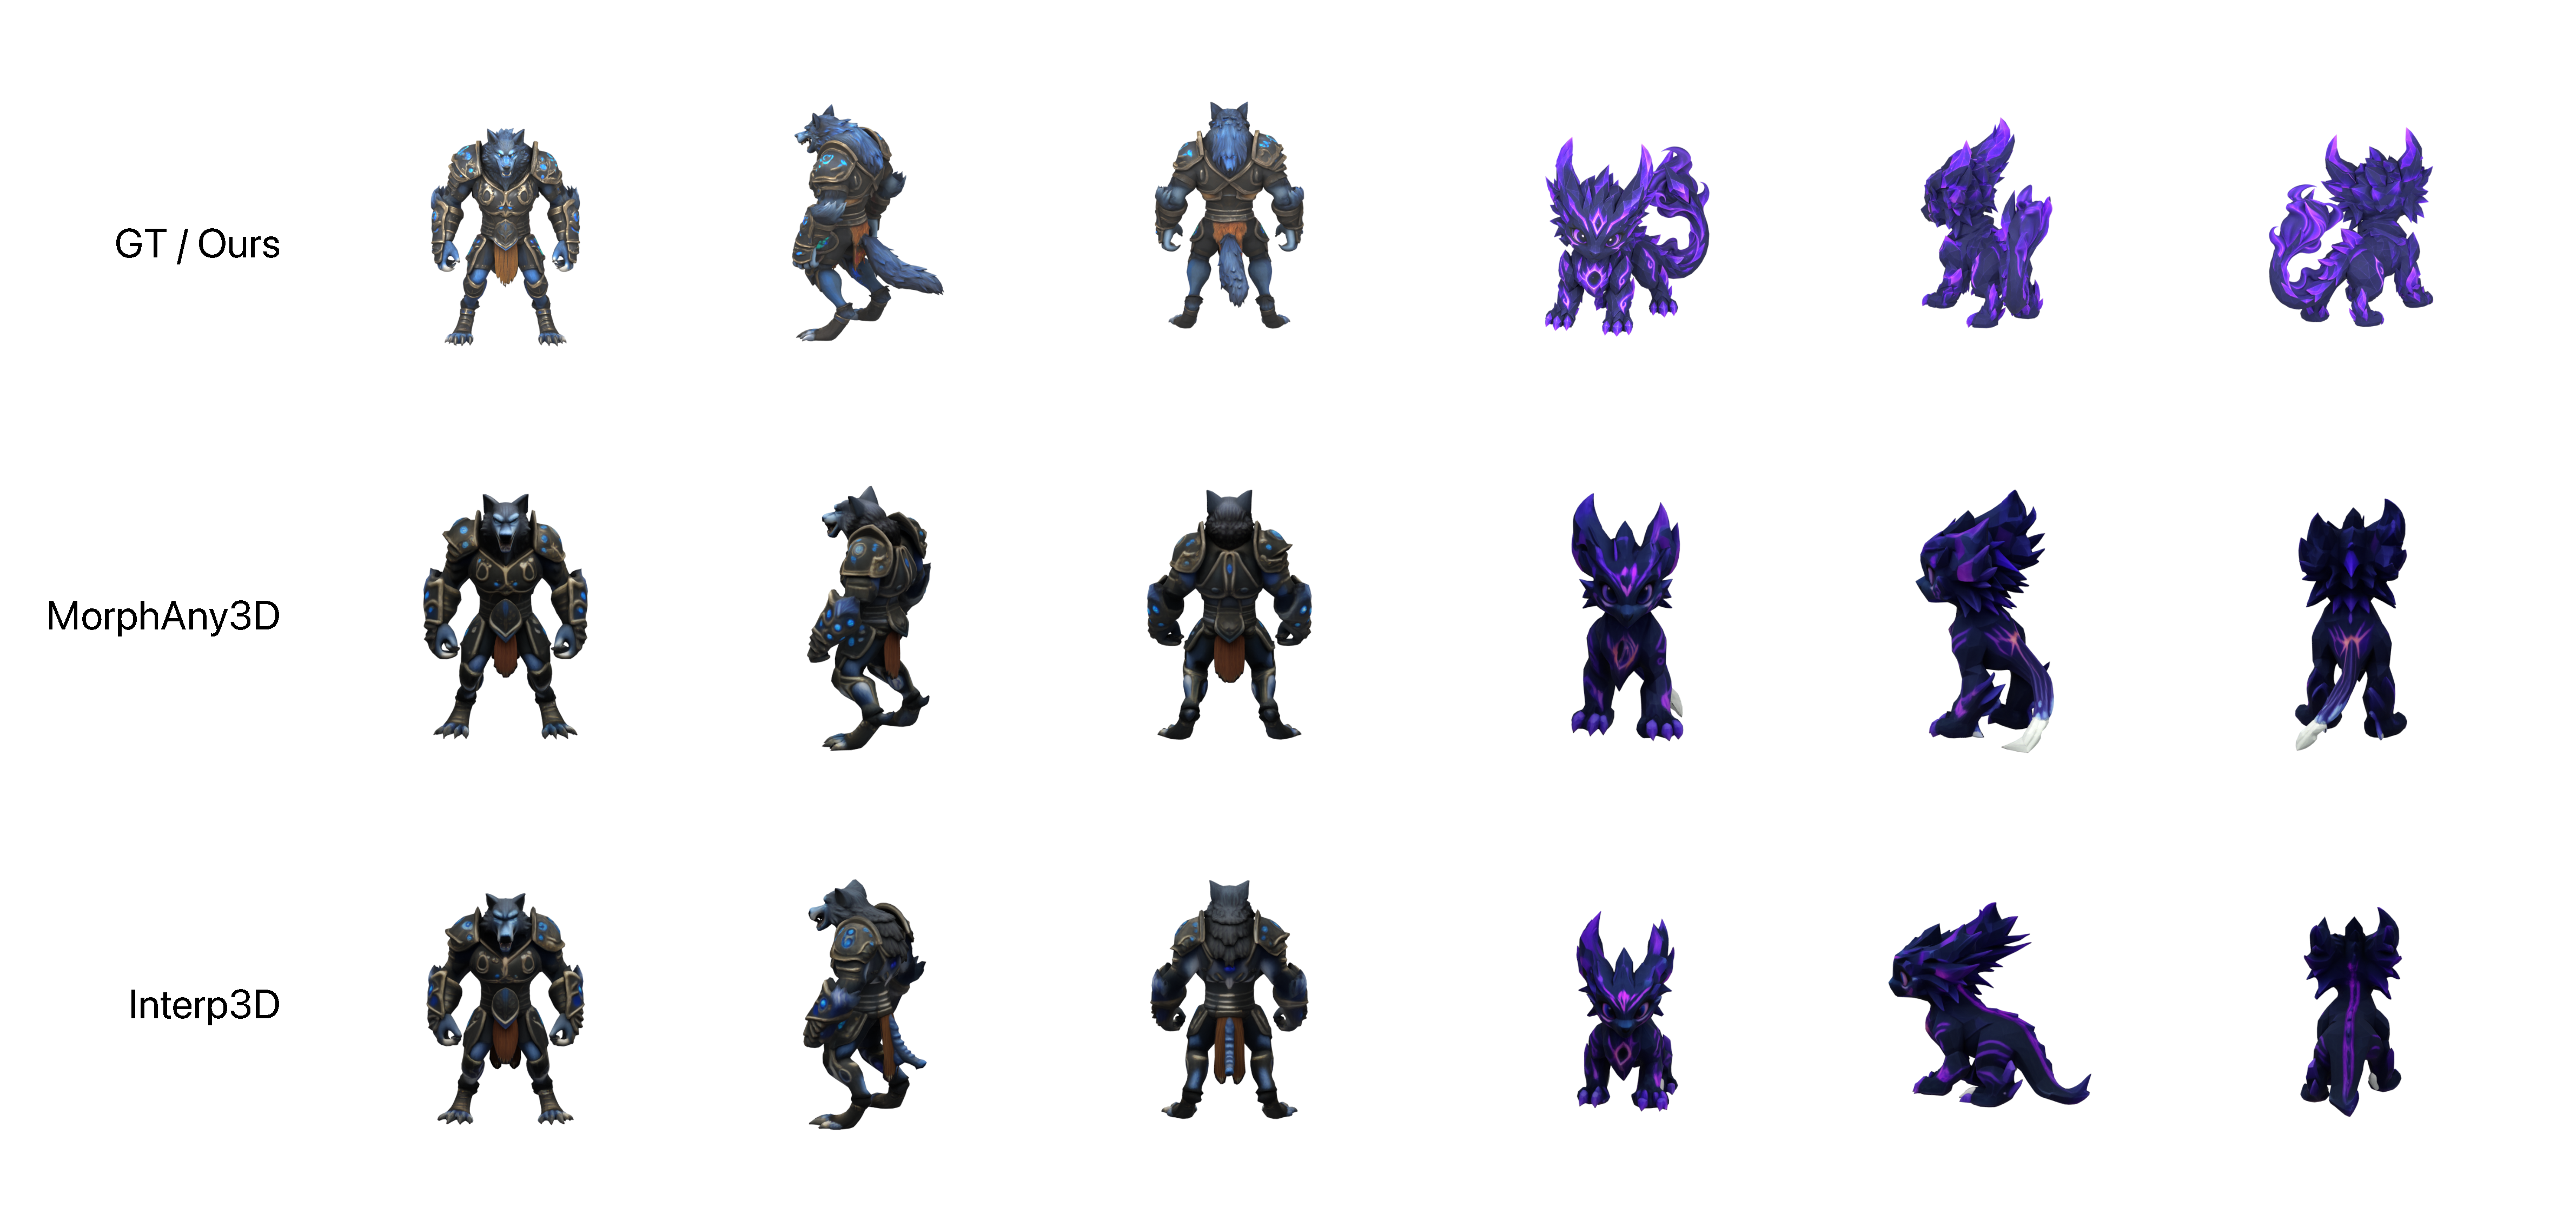
\includegraphics[width=\columnwidth]{figures/comparison_errors.pdf}
%  \caption{todo}
%  \label{fig:comparison_errors}
% \end{figure}


% \subsection{Ablations}
% \label{sec:ablations}

% The ablation study uses the Interp Protocol to test whether the prior improves FID and
% gating reduces PDV. The full model targets a balance between source
% fidelity and transition quality. Table~\ref{tab:ablation} awaits
% matched-step results.

% \begin{table}[t]
\centering
\small
\setlength{\tabcolsep}{5pt}
\caption{Ablations under the Interp Protocol. Baseline disables gate, prior, and source swap; component variants enable only the named term, and Full Model uses all three. Final matched-step measurements are pending.}
\label{tab:ablation}
\begin{tabular}{lrrrr}
\toprule
Variant & FID $\downarrow$ & PPL $\downarrow$ & PDV $\times10^3\!\downarrow$ & EPRE $\downarrow$ \\
\midrule
Baseline & 96.54 & \second{3.55} & 0.90 & 0.26 \\
Gate Only & 102.34 & \best{3.54} & \best{0.84} & 0.26 \\
Prior Only & \best{91.17} & 3.58 & 0.91 & 0.26 \\
Full Model & \second{95.03} & 3.58 & \second{0.85} & 0.26 \\
\bottomrule
\end{tabular}
\end{table}


\section{Conclusion}
\label{sec:conclusion}

\methodname{} è la migliore

\subsection{Limitations}
\label{sec:limitations}

consistenza non è imposta con una loss, possibile idea per futuro


% Keep result figures and tables ahead of the bibliography.
\clearpage
{
    \raggedbottom
    \small
    \bibliographystyle{ieeenat_fullname}
    \bibliography{main}
}

% WARNING: do not forget to delete the supplementary pages from your submission 
% \clearpage
\setcounter{page}{1}
\maketitlesupplementary


\section{Rationale}
\label{sec:rationale}
% 
Having the supplementary compiled together with the main paper means that:
% 
\begin{itemize}
\item The supplementary can back-reference sections of the main paper, for example, we can refer to \cref{sec:intro};
\item The main paper can forward reference sub-sections within the supplementary explicitly (e.g. referring to a particular experiment); 
\item When submitted to arXiv, the supplementary will already included at the end of the paper.
\end{itemize}
% 
To split the supplementary pages from the main paper, you can use \href{https://support.apple.com/en-ca/guide/preview/prvw11793/mac#:~:text=Delete%20a%20page%20from%20a,or%20choose%20Edit%20%3E%20Delete).}{Preview (on macOS)}, \href{https://www.adobe.com/acrobat/how-to/delete-pages-from-pdf.html#:~:text=Choose%20%E2%80%9CTools%E2%80%9D%20%3E%20%E2%80%9COrganize,or%20pages%20from%20the%20file.}{Adobe Acrobat} (on all OSs), as well as \href{https://superuser.com/questions/517986/is-it-possible-to-delete-some-pages-of-a-pdf-document}{command line tools}.

\end{document}
